\documentclass[12pt,a4paper]{article}
\usepackage[utf8]{inputenc}
\usepackage[spanish]{babel}
\usepackage{amsmath}
\usepackage{amsfonts}
\usepackage{amssymb}
%\\usepackage[left=3cm,right=3cm,top=3cm,bottom=3cm]{geometry}		%para los márgenes
\usepackage{enumerate}	%para enumerar
\usepackage{lscape}		%para poner una página en horizontal
\usepackage{pdfpages}	%para incluir pdf
\usepackage{eurosym}		%para el símbolo del euro
\usepackage{emptypage}	%para que no aparezca encabezado en las páginas en blanco
\usepackage{fancyhdr}	%paquete para encabezado
\usepackage{lastpage}
\usepackage[hidelinks]{hyperref}		%para el índice con hipervínculos
\usepackage{float}
\usepackage{subfig}
\graphicspath{ {images/} }	%ruta de las imágenes



\cfoot{\thepage}
%\renewcommand{\headrulewidth}{0pt} 	%define el grosorde la línea

\begin{document}

% PORTADA
\begin{titlepage}
\begin{center}
% línea antes del título
\rule{80mm}{0.1mm}\\		%\rule{ancho}{alto}
\bigskip
% título de la portada
\begin{Huge}
\textsc{Genetic Tuning on Fuzzy Systems Based on the Linguistic 2-Tuples Representation\\}
\end{Huge}
% línea después del título
\bigskip
\rule{80mm}{0.1mm}\\		%\rule{ancho}{alto}
\bigskip

\includegraphics[scale=0.4]{Portada/logoUHU}\\
\bigskip
\bigskip
\Large
\textbf{Inteligencia computacional}\\
\bigskip
\bigskip
\bigskip
\bigskip
\bigskip
\bigskip
Profesor: Francisco Alfredo Márquez Hernández y Antonio Peregrín Rubio.\\
Alumnos: Ana Godoy Pérez y José Manuel López Betanzos\\
\bigskip
\bigskip
\bigskip
Máster en Ingeniería Informática\\
Escuela Politécnica Superior de Ingeniería\\
Universidad de Huelva\\
\end{center}
\end{titlepage}


\thispagestyle{empty}
% ÍNDICE
\tableofcontents
%Cambiar nombre del indice
\renewcommand{\contentsname}{Índice}
%Indicar la profundidad
\setcounter{tocdepth}{3}
\newpage


% CONTENIDO
\part*{Objetivos}
El objetivo de esta práctica es la creación de un software que permita el diseño y lanzamiento de un controlador difuso MISO (Multiple input Simple Output) sobre un conjunto de valores de variables, que además permita un aprendizaje de las etiquetas lingüísticas (tuning) sobre un fichero de entrenamiento.

\section{Creación de un Software para el diseño y lanzamiento de un Controlador Difuso de Tipo Mamdani}
En esta primera parte se pretender crear un software que permita el diseño y lanzamiento de un controlador difuso de tipo Mandani. Este software permitirá definir el número de variables de entrada, la variable de salida, el universo de discurso, el número de etiquetas lingüísticas para cada una de las variables, así como el operador de implicación, conjunción y el método de inferencia. Además permitirá introducir una base de reglas en un formato
predefinido.
Para simplificar esta primera parte se utilizarán etiquetas triangulares. Además, como operadores de
conjunción e implicación la t-norma del mínimo y como método de defuzzificación un Modo B.

A continuación se van a explicar los paquetes de los que está compuesto este software, que se corresponden con los componentes forman un sistema difuso de este tipo: base de conocimiento, interfaz de fuzzificación, sistema de inferencia e interfaz de defuzzificación. Asímismo cuenta con otros paquetes auxiliares que ayudarán a cargar los datos necesarios en el sistema. Todos ellos cuenta con su JavaDoc y el código está comentado para facilitar la compresión del mismo.

También es necesario tener en consideración que la relación entre las partes del sistema será la mostrada en la siguiente imagen \ref{flujoFS} :
\begin{figure}[H]
\centering
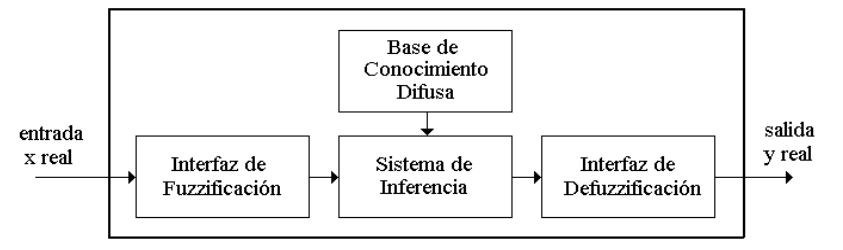
\includegraphics[width=0.8\textwidth]{flujoFS}
\caption{Flujo de un sistema difuso de tipo Mamdani.}
\label{flujoFS}
\end{figure}

\subsection{Base de conocimiento}
La base de conocimiento almacena el conocimiento particular del problema a resolver. Consta de dos elementos: la base de reglas y la base de conocimiento. Tanto la estructura de datos de la BC como la información que la formará debe ser especificada antes de que el SBRD comience a funcionar.

\begin{figure}[H]
\centering
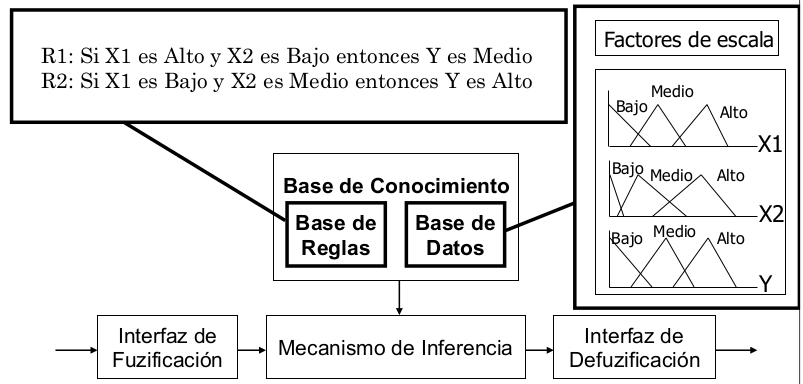
\includegraphics[width=0.8\textwidth]{baseConocimiento}
\caption{Base de conocimiento del sistema difuso.}
\label{flujoFS}
\end{figure}

\subsubsection{Base de Datos}
La base de datos contiene la definición de los conjuntos difusos asociados a los términos lingüísticos empleados en las reglas de la BR.\\
Para su definición se ha optado por una tabla hash en la que cada valor queda definido por el triángulo que representa a una partición difusa del conjunto difuso de las variables. Este ''triángulo'' no sólo almacena las coordenadas de la etiqueta si no que también almacena a qué variable del conjunto difuso pertenece. Como key de la tabla hash se empleará un número en el intervalo [1,num$\_$etiquetas].\\
Los datos necesarios para dar contenido a esta estructura serán tomados del fichero con extensión \textit{.pwm}

\subsubsection{Base de Reglas}
La base de reglas está formada por un conjunto de reglas lingüísticas de tipo ''Si - entonces''. En este caso las reglas contenidas en el fichero de extensión \textit{.wm} vienen definidas por las coordenadas de las etiquetas a las que hacen referencia.\\
Cada regla será almacenada como el conjunto de referencias a las etiquetas que la forman.

\subsection{Interfaz de fuzzificación}
Este componente es uno de los que permite al SBRD de tipo Mamdani manejar entradas y salidas reales. Su tarea es la de establecer una aplicación que haga corresponder un conjunto difuso, definido en el universo de discurso de la entrada en cuestión, a cada valor preciso del espacio de entrada.\\
Para almacenar esta correspondencia se ha optado de nuevo por una tabla hash que tendrá por clave la variable de entrada que se está considerando, y como valor las referencias a las particiones difusas (etiquetas) a las que pertenece.

\subsection{Sistema de inferencia}
El Sistema de Inferencia es el componente encargado de llevar a cabo el proceso de inferencia difusa. Para ello el Sistema de Inferencia deberá realizar las siguientes tareas sobre cada regla de la Base de Reglas:
\begin{itemize}
\item Determinar $\mu_{A}(x_{0})$, mediante el Operador de Conjunción (en esta práctica se empleará el mínimo).El resultado, denominado grado de emparejamiento (en adelante lo notaremos por h) de dichas entradas con la regla que se está evaluando, representa una medida de ''coincidencia'' de los valores que toman las variables de
entrada con los valores lingüísticos que describen el antecedente de esa regla. Estos valores se irán almacenando en el array \textit{matching} para su posterior uso.
\item Aplicar del Operador de Implicación, F (en esta práctica se empleará el mínimo). En el caso que nos ocupa, debido a que sólo existirá un consecuente, F = min, es decir, directamente se guardará el punto de máximo valor de la variable de salida del consecuente de la regla que se está evaluando en el vector \textit{pmv}.
\end{itemize}

\subsection{Interfaz de defuzzificación}
Convierte la salida del sistema de inferencia (lo inferido por cada regla) en un único valor real final. En este caso el método que se empleará para calcular este valor único será el Modo B, que consiste en convertir la aportación de cada regla en un número, que en esta práctica se ha hecho mediante el PMV (punto de máximo valor) y calcular un único valor final como salida empleando la siguiente fórmula: 
\begin{figure}[H]
\centering
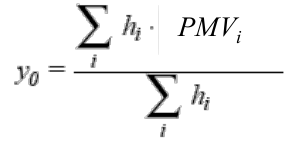
\includegraphics[width=0.3\textwidth]{salida}
\label{flujoFS}
\end{figure}

\subsection{Read}
Este paquete cuenta con las clases necesarias tanto para leer la información relativa al problema y almacenarla en  las estructuras correspondientes, como para escribir las salidas en el formato deseado.\\
A continuación se explica la finalidad de cada una de ellas:
\begin{itemize}
\item \textbf{ReadPWM:} lee un fichero de extensión .pwm que contiene la información relativa a la base de datos y la almacena.
\item \textbf{ReadRB:} lee un fichero de extensión .wm  que contiene las reglas que definen al sistema difuso. Este fichero también contiene la salida por defecto y el error cuadrático medio de los fichero tanto de training como de test.
\item \textbf{ReadExamples:} lee un fichero de training o test y guarda las entradas y salidas en dos estructuras respectivamente. Además esta clase permite calcular el error cuadrático medio del fichero leído, así como calcular las salidas para un conjunto de valores de entradas. También permite escribir las salidas obtenidas tras el entrenamiento o la fase de test siguiendo la estructura de estos ficheros.
\end{itemize}

\subsection{Files}
El paquete Files contiene los ficheros necesarios para la ejecución del sistema fuzzy: base de datos (.pwm), base de reglas (.wm), fichero de entrenamiento (.tra) y test (.tst). También albergará las salidas producidas tras una ejecución.

\subsection{FuzzySystem}
Este paquete contiene tanto la clase principal que contiene al \textit{main()}, como una clase en la que se han almacenado los parámetros que se emplearán a lo largo de todo el sistema.


\subsection{Ejecución del software}
Para ejecutar el software habrá que moverse a la carpeta \textit{FuzzySystem/dist}. Esta carpeta deberá contener el \textit{.jar} y la carpeta \textit{src/Files} con al menos los siguientes archivos: base de reglas, base de datos y fichero de entrenamiento. Además, esta carpeta contará con un README.TXT en el que se explica cómo ejecutar el software.\\
El controlador difuso se puede lanzar de dos formas:
\begin{itemize}
\item Dando un ejemplo de entrada, en cuyo caso devolverá la salida que quedará almacenada en \textit{src/Files/Output.txt}. La instrucción para ejecutar esta opción sería:
\begin{center}
\textit{java -jar "FuzzySystem.jar" -in valor1 valor2 valori}
\end{center}
\item Dando un fichero de entrenamiento \textit{.tra} con una secuencia de valores de entrada salida (una línea por cada secuencia), en cuyo caso cogerá por cada línea del fichero de entrenamiento los valores de las variables de entrada y devolverá los valores de la ejecución del controlador. Además, devolverá el error cuadrático medio (ECM). La salida de esta ejecución se almacenará en \textit{src/Files/Output$\_$tra.txt} siguiendo el mismo formato que el que tiene el fichero de entrenamiento. 
\begin{center}
\textit{java -jar FuzzySystem.jar -tra ruta$\_$del$\_$fichero.tra}
\end{center}
\end{itemize}



\section{Ampliación del Software para realizar un aprendizaje de etiquetas linguisticas (tuning)}
Esta ampliación del software permitirá realizar un ajuste paramétrico de las etiquetas lingüísticas de las variables. Para ello se implementará un ajuste mediante un Algoritmo Genético basado en el ajuste de 2-tuplas.
El ajuste se realizará minimizando el ECM de cada posible solución con el fin de obtener después de diversas generaciones la solución más óptima.\\
El algoritmo genético empleado es el CHC con los parámetro recomendados en el enunciado de la prática:
\begin{itemize}
\item Tamaño de población: 50
\item Operador de Cruce: BLX-alpha (alpha=0.5)
\item Probabilidad de Cruce: CHC (1.0)
\item Criterio de parada: 200 iteraciones
\end{itemize}

\subsection{Construcción del algoritmo CHC}
Para construir el algoritmo se han seguido los pasos expuestos en el Tema 2.3 de la asignatura Metahurística cursada en el 4º curso de Grado en Ingeniería Informática. Esos pasos se detallan a continuación:

\subsubsection{Diseñar una representación}
Cada individuo utilizará una representación real, en la que cada cromosoma tendrá la siguiente forma (donde cada gen está asociado al valor de tuning de la etiqueta correspondiente):
\begin{center}
$(c_{11},...,c_{1m^{1}},c_{21},...,c_{2m^{2}},...,c_{n1},...,c_{nm^{n}})$
\end{center}
Considerando el siguiente número de etiquetas por variables $(m^{1},m^{2},...,m^{n})$, siendo n el número de variables.
\begin{figure}[H]
\centering
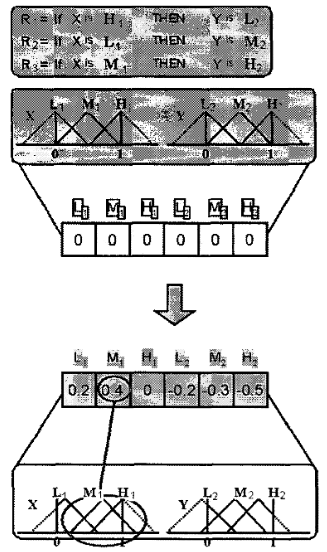
\includegraphics[width=0.4\textwidth]{individuo}
\caption{Codificación de un cromosoma.}
\label{individuo}
\end{figure}

\subsubsection{Decidir como iniciar (reiniciar) una población}
La población (que representará un conjunto de soluciones) se inicializará creando tantos individuos de forma aleatoria, en el intervalo [-0.5,0.5], como tamaño tenga la población, a excepción de uno, que inicializará su cromosoma a cero, es decir, no realizando ningún tuning sobre el conjunto difuso. Este individuo representará la ''solución base''.\\
La reinicialización o multiarranque en CHC es empleada como mecanismo para producir una alta diversidad alejándose de óptimos locales. Este mecanismo se utilizará cuando el umbral de cruce sea menor que cero, manteniendo al mejor individuo y generando el resto de la población de forma aleatoria. El umbral se inicializa a L/4, siendo L la longitud del cromosoma.

\subsubsection{Diseñar una forma de evaluar a un individuo}
Para evaluar a un cromosoma se utilizará el error cuadrático medio (ECM):
\begin{center}
$MSE = \dfrac{1}{2 \cdot N} \sum_{l=1}^{N}(F(x^{l}) - y^{l})^{2}$
\end{center}
Siendo N el número de ejemplos, $F(x^{l})$ la salida obtenida por el sistema difuso tras aplicarle el tuning e $y^{l}$ la salida conocida.

\subsubsection{Diseñar un operador de cruce adecuado}
El operado de cruce empleado en esta práctica es el $BLX-\alpha$ con $\alpha = 0.5$.

\subsubsection{Decidir cómo seleccionar a los individuos para ser padres}
Se forman N/2 parejas con los elementos de la población (siendo N el tamaño de la población). Sólo se cruzan las parejas cuyos miembros difieren en un número determinado de bits (umbral de cruce). Si durante un
ciclo no se produce ni un solo cruce, al umbral de cruce se le resta 1.

\subsubsection{Decidir cómo reemplazar a los individuos}
Se empleará la selección elitista como método de reemplazamiento. Este método selecciona los N mejores cromosomas entre padres e hijos.

\subsubsection{Decidir la condición de parada}
La condición de parada se ha establecido como que se cumplan un número determinado de iteraciones. Para determinar este número se han realizado tres ejecuciones, incrementando en cada una de ellas el número de iteraciones en el rango [100,300].\\\\

\begin{tabular}{|c|c|c|}
\hline 
Iteraciones & ECMtra & ECMtst \\ 
\hline 
100 & 211647.18644149418 & 189450.95883628397 \\ 
\hline 
200 & 211641.61045261426 & 189448.078221798 \\ 
\hline 
300 & 211641.54301892893 & 189448.03784438976 \\ 
\hline 
\end{tabular} 
~\\
~\\
De acuerdo a los resultado el número de iteraciones establecido como criterio de parada es 200.


\subsection{Ejecución del software}
Para ejecutar el software habrá que moverse a la carpeta \textit{GAFuzzySystem/dist}. Esta carpeta deberá contener el \textit{.jar} y la carpeta \textit{src/Files} con al menos los siguientes archivos: base de reglas, base de datos y ficheros y test de entrenamiento. Además, esta carpeta contará con un README.TXT en el que se explica cómo ejecutar el software.\\
El controlador difuso con ajuste del conjunto difuso mediante el algoritmo CHC se puede lanzar de dos formas:
\begin{itemize}
\item Dando un fichero \textit{.tra} que ejecutará el algoritmo CHC para realizar el tuning de la base de datos.
Esta ejecución producirá como salida un fichero \textit{src/Files/BaseDatos.pwm} con la nueva base de datos resultado de aplicar los desplazamientos indicados por el mejor cromosoma de la población tras la ejecución del algoritmo. Asimismo creará un fichero con la base de reglas con las etiquetas de las reglas actualizadas a los nuevos valores que se guardará como \textit{src/Files/BaseReglas.wm}. Además creará el fichero \textit{src/Files/Output$\_$tra.txt} que recogerá las salidas del fichero de entrenamiento y el ECM. La instrucción para ejecutar esta opción sería:
\begin{center}
\textit{java -jar "GAFuzzySystem.jar" -tra ruta$\_$fichero$\_$entrenamiento.tra ruta$\_$base$\_$datos.pwm}
\end{center}
\item Dando un fichero de test \textit{.tst}, que tomará la base de datos y la base de reglas obtenida en el entrenamiento, con una secuencia de valores de entrada salida (una línea por cada secuencia), en cuyo caso cogerá por cada línea del fichero de entrenamiento los valores de las variables de entrada y devolverá los valores de la ejecución del controlador. Además, devolverá el error cuadrático medio (ECM). La salida de esta ejecución se almacenará en \textit{src/Files/Output$\_$tst.txt} siguiendo el mismo formato que el que tiene el fichero de test. 
\begin{center}
\textit{java -jar "GAFuzzySystem.jar" -tst ruta$\_$fichero$\_$test.tst ruta$\_$base$\_$datos$\_$tuning.pwm}
\end{center}
\end{itemize}

\end{document}


